\documentclass[PMO,lsstdraft,authoryear,toc]{lsstdoc}
% lsstdoc documentation: https://lsst-texmf.lsst.io/lsstdoc.html
% \input{meta}

% Package imports go here.

% Local commands go here.

%If you want glossaries
%\input{aglossary.tex}
%\makeglossaries

\title{Third Floor Network Planning}

% Optional subtitle
% \setDocSubtitle{A subtitle}

\author{Guido Maulen, Julio Constanzo, Hernán Stockebrand 
}

\setDocRef{ITTN-047}
\setDocUpstreamLocation{\url{https://github.com/lsst-it/ittn-047}}

\date{\today}

% Optional: name of the document's curator
% \setDocCurator{The Curator of this Document}

\setDocAbstract{%
The following document details the plan to deploy the fibers, devices, and configuration to provide a solution for the connectivity on the third-floor laboratories at the Vera C. Rubin building at Pachon Mountain. 
}

% Change history defined here.
% Order: oldest first.
% Fields: VERSION, DATE, DESCRIPTION, OWNER NAME.
% See LPM-51 for version number policy.
\setDocChangeRecord{%
  \addtohist{1}{2021-06-16}{Unreleased.}{Hernan Stockebrand}
}


\begin{document}

% Create the title page.
\maketitle
% Frequently for a technote we do not want a title page  uncomment this to remove the title page and changelog.
% use \mkshorttitle to remove the extra pages

% ADD CONTENT HERE
% You can also use the \input command to include several content files.

\section{Introduction}


The following documentation provides a closer look at network installation on the third-floor labs while providing an inside look at the materials used and areas involved. The IT Team at Rubin is in charge of installing the fiber optic cable that originates at the computer room located on the second floor of the main building and extending to the fiber distribution box that will be installed on the third floor, any other connections related to this activity will be carried out by other Rubin Staff members.



The IT requirements are the following:

Install 6 pair single mode fibers and 6 pair multimode fibers from the Computer room to the fiber boxes that needs to be installed on the third floor	
The cables used for this project were OS2 LC Full duplex and OM3 LC Full duplex

\newpage
\section{Proposed Layout}

\begin{figure}
  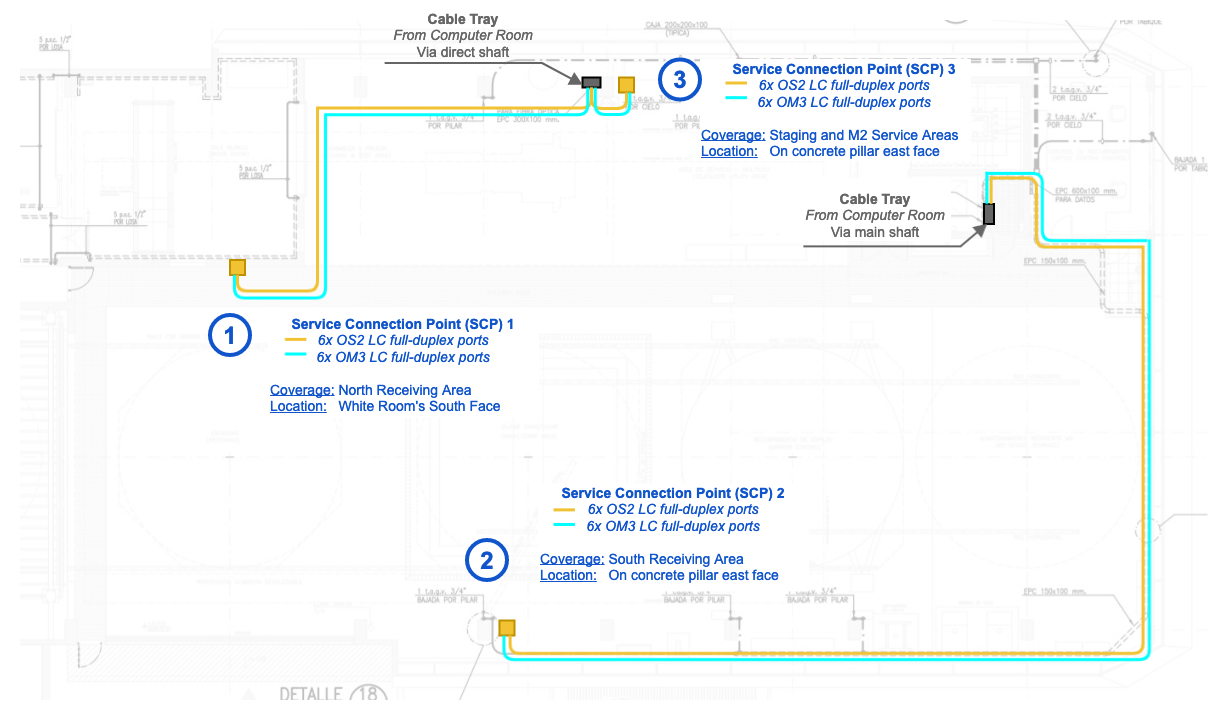
\includegraphics[width=16cm]{images/image-001.png}
  \centering
  \caption{Proposed layout}
\end{figure}

\subsection{Explanation}

As the images describes, is possible to watch the proposed location of the SCP around the laboratories at the thir floor, where each cabinet will contain inside a PDU, UPS and a Gigabit Switch.
also it will be possible to move at least few meter the rack from the SCP, with fiber and power extension rolled on a reel assembly

\newpage
\section{Network configuration}
  \subsection{High Level Topology}
  \begin{figure}
    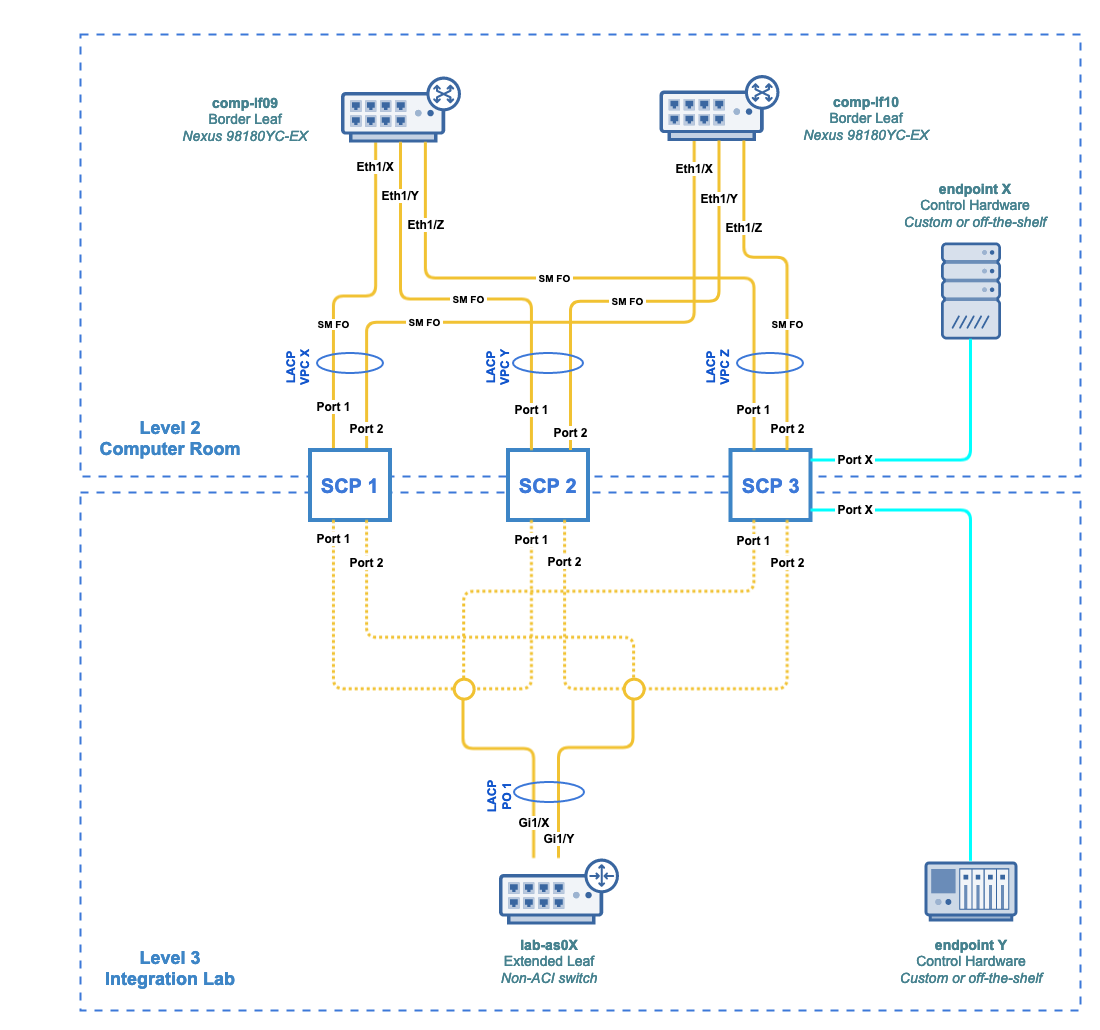
\includegraphics[width=14cm]{images/image-002.png}
    \centering
    \caption{Network configuration High level topology}
  \end{figure}

  \newpage
  \subsection{Explanation}
    The above diagram represents the concept of the "always-on" connections to be implemented. 
    The idea is to have a pair of interfaces in the ACI border leafs pre-configured and always cabled up for this purpose, each pair of interfaces connect to the Service Connection Points (SCP) in such way that the switches used for integration at Level 3 can physically roam around the floor and the engineers working in the area can get the connection back online only by moving the fibers to the exact same ports in the next SCP. 
    The diagram shows only 1 switch but there will be installed one Kit ( i.e. Mobile Rack, Gigabit Switch, UPS, PDU and Reel asembly) per SCP
    For network connections you will want to use single-mode all the time to future proof the install in case of special integration requirements that ask for more bandwidth


    Some relevant points to have in consideration for the implementation:
    \begin{itemize}
      \item All vPCs on the datacenter side should be configured in the same way for this to work properly and without IT intervention.
      \item The fabric will see the endpoints mac-addresses "flapping" from one port to another and Syslog may alert about this; this is expected but be careful with false-positives when it comes to monitoring and alerting.
      \item Label everything properly and provide the non-IT engineers with specific instructions for moving a switch from one SCP to another.
    \end{itemize}

 \newpage
\section{Bill of Materials}

\begin{flushleft}\begin{tabular}{|c|c|c|c|c|}
  \hline
  Qty & Part Number & Part Name & Vendor & Comments \\ 
  \hline
  3 &  & Gigabit Switch &  & 16 Ports 1GB \\ 
  \hline
  3 &  & Steel Rack 12RU  &  & with 3" Casters  \\ 
  \hline
  3 & 5WSML-2C & SDX Wall-Mount Fiber  & Leviton    \\ 
  \hline
  3	& SPLMT-HKT	& Splice tray mount kit	& Leviton  \\
  \hline
  3	& 5L000-KAL	& Lock for Wall-Mount Fiber 	& Leviton  \\
  \hline
  2	& 5R1UM-S03	1000i & SDX 19-inch Fiber 	& Leviton  \\
  \hline
  12 &	T5PLS-12F	& Splice tray for 12 fibers	& Leviton \\
  \hline
  144	& N/A	& 40mm splice sleeve	& FS or generic	 \\
  \hline
  72	& N/A	& 1m OS2 LC pigtail	& FS or generic  \\
  \hline
  72 &	N/A	& 1m OM3 LC pigtail	& FS or generic \\
  \hline
  6	& P03404	& 6x port SM OS2 LC & fiber plate	Trimerx  \\
  \hline
  6	& P03397	& 6x port MM OM3 LC & fiber plate	Trimerx  \\
  \hline
  350m && Nexo DT 24 fibers OS2	& Optral  \\
  \hline
  350m && Nexo DT 12 fibers OM3	& Optral \\
  \hline
  \end{tabular}\end{flushleft}


\newpage

\section{Bill of Materials}

\begin{tabular}{|c|c|c|c|c|}
  \hline
  Qty & Part  & Specification &  Comments \\ 
  \hline


  1 & Network Switch & 24 Ethernet Ports &  SFP Uplinks \\ 
  \hline

  3 & Server Rack Cabinet& 12U & with 3" Casters  \\ 
  \hline

  8 & LC-LC OS2 SM & 20m & Indstrial Grade  \\ 
  \hline

  2 & LC-LC OS2 SM & 30m & Indstrial Grade  \\ 
  \hline

  2 & LC-LC OM3 MM & 30m & Indstrial Grade  \\ 
  \hline

  30 & LC-LC OS2 SM & 5m & Indstrial Grade  \\ 
  \hline

  30 & LC-LC OM2 MM & 5m & Indstrial Grade  \\ 
  \hline

    
  3 &  UPS & 1000kva 110v   &  \\ 
  \hline
  
  3 & Cable Roller  &   &     \\ 
  \hline


  \end{tabular}
\newpage

\section{Deployment Plan}

Our deployment plan will begin once the new cable trays are installed in the laboratory, then the fiber installation from the Datacenter to the SCP will begin.
Once installed the SCP, the fiber technician will fusion the fibers kind of connections on the pre-defined points.
The following steps are to assemble the racks with the installation of the devices, including his logical configurations.


The installation of this equipment will require the help of a group of 4 people, and work will carry out throughout four days, 
taking into fiber install two days, one day to assemble de racks, and one day for logical configuration. 

\subsection{Deployment Conclusions and Considerations}

\begin{itemize}
    \item Wait around 2 months for the materials to be delivered and have them at the summit.
    \item All cable installation work must be coordinated one week in advance.
\end{itemize}





\appendix
% Include all the relevant bib files.
% https://lsst-texmf.lsst.io/lsstdoc.html#bibliographies
\section{References} \label{sec:bib}
\renewcommand{\refname}{} % Suppress default Bibliography section
\bibliography{local,lsst,lsst-dm,refs_ads,refs,books}

% Make sure lsst-texmf/bin/generateAcronyms.py is in your path
\section{Acronyms} \label{sec:acronyms}
\addtocounter{table}{-1}
\begin{longtable}{p{0.145\textwidth}p{0.8\textwidth}}\hline
\textbf{Acronym} & \textbf{Description}  \\\hline

IT & Information Technology \\\hline
PDU & Power Distribution Unit \\\hline
PMO & Project Management Office \\\hline
UPS & uninterruptible power supply \\\hline
\end{longtable}

% If you want glossary uncomment below -- comment out the two lines above
%\printglossaries





\end{document}
